%----------------------------------------------------------------------------------------
%    PACKAGES AND THEMES (your CleanEasy template)
%----------------------------------------------------------------------------------------
\documentclass[aspectratio=169,xcolor=dvipsnames]{beamer}
\makeatletter
\def\input@path{{theme/}}
\makeatother
\usetheme{CleanEasy}

\usepackage[utf8]{inputenc}
\usepackage{lmodern}
\usepackage[T1]{fontenc}
% \usepackage[brazil]{babel}
\usepackage{fix-cm}
\usepackage{amsmath}
\usepackage{mathtools}
\usepackage{amssymb} % added for \mathbb etc.
\usepackage{listings}
\usepackage{xcolor}
\usepackage{hyperref}
\usepackage{graphicx}
\usepackage{booktabs}
\usepackage{tikz}
\usetikzlibrary{positioning, shapes, arrows, calc, decorations.pathreplacing, arrows.meta, backgrounds, patterns, overlay-beamer-styles}
\usepackage{etoolbox}
\usepackage{animate}
\usepackage{multirow}
%----------------------------------------------------------------------------------------
%    LAYOUT CONFIGURATION (from your theme)
%----------------------------------------------------------------------------------------



% Configure code listings
\lstset{
  basicstyle=\ttfamily\small,
  keywordstyle=\color{blue},
  commentstyle=\color{green!60!black},
  stringstyle=\color{red},
  showstringspaces=false,
  breaklines=true,
  frame=single,
  rulecolor=\color{black!30},
  backgroundcolor=\color{black!5},
  numbers=left,
  numberstyle=\tiny\color{black!70},
  numbersep=5pt
}

%---------------------------------------------
\title[Ropeformer: Cross-Attention]{Cross-Attention Transformers with ROPE for Oil Index Forecasting}

\author[Y. Liu]{Yuncong Liu}

\institute[NUS]{Department of Mathematics \\
National University of Singapore}

\date{Oct 6, 2025}

% Titlegraphic left empty (no corner logos)
\titlegraphic{}

%----------------------------------------------------------------------------------------
%    Your shorthands (kept from your original)
%----------------------------------------------------------------------------------------
\newcommand{\hist}{L}
\newcommand{\dmodel}{d}
\newcommand{\din}{C}
\newcommand{\fnum}{M}

% --- colors & helpers ---
\usepackage{xcolor}
\definecolor{ShortColor}{RGB}{33,113,181}   % 蓝：短期
\definecolor{MidColor}{RGB}{35,139,69}      % 绿：中期
\definecolor{LongColor}{RGB}{178,34,34}     % 红：长期

\newcommand{\shortf}[1]{\textcolor{ShortColor}{#1}}
\newcommand{\midf}[1]{\textcolor{MidColor}{#1}}

% --- colours used by the new result slides ---
\definecolor{navy}{HTML}{0D2659}
\definecolor{blockhead}{HTML}{045073}
\definecolor{blockbody}{HTML}{EBEBF7}
\definecolor{alertbody}{HTML}{F7EBEB}
\definecolor{fixedc}{HTML}{EB6834}
\definecolor{learnc}{HTML}{2A78D6}
\makeatletter\let\inputtab\@@input\makeatother

%----------------------------------------------------------------------------------------
%    TITLE
%----------------------------------------------------------------------------------------
\title[Learning the Rhythm: RoPE beyond the training horizon]{Learning the Rhythm: Why RoPE Degrades Beyond the Training Horizon, and How Learnable Frequencies Help}
\author[Liu, Zhang, Ma]{Liu Yuncong \quad Zhang Yihang \quad Ma Xiaoyu}
\institute[NUS]{FT5011 Deep Learning for Finance \\ National University of Singapore}
\date{11 November 2026}

\begin{document}

% ===== Title & TOC =====
\begin{frame}[plain]
  \titlepage
\end{frame}

\begin{frame}[plain]{Contents}
  \tableofcontents
\end{frame}

% ===================== Problem & Background =====================
\section{Problem \& Background}

\begin{frame}{Problem: one model, many horizons}
\textbf{Finance needs forecasts at several horizons at once.}
\begin{itemize}
\item Risk: Value-at-Risk at \textbf{1 day} and \textbf{10 days}; volatility daily $\to$ weekly $\to$ monthly (HAR).
\item Energy trading: bid for \textbf{tomorrow}, hedge for \textbf{next week}.
\item Usual practice: \emph{one model per horizon} --- costly to train and maintain.
\end{itemize}
\begin{block}{Goal}
Train once on a short horizon, then forecast \textbf{any} horizon:
\[
\underbrace{x_{t-335},\dots,x_t}_{L=336\ \text{past steps}}
\;\longmapsto\;
\underbrace{\hat x_{t+1},\dots,\hat x_{t+H'}}_{\text{trained with } H=96,\ \text{asked for } H'\le 720}
\]
\end{block}
\small A \textbf{step} = one observation. On hourly prices, 96 steps = \textbf{4 days}, 720 steps = \textbf{30 days}.
\end{frame}

\begin{frame}{The problem: silent failure beyond the training horizon}
\begin{columns}[T]
\column{0.6\textwidth}
\textbf{What happens.} Trained for 96 steps (4 days), asked for 720 (30 days): the error rises sharply beyond the training horizon.

\smallskip
\textbf{Why it matters.}
\begin{itemize}
\item \textbf{Silent}: fine at the training horizon, no warning beyond it.
\item \textbf{Common}: RoPE is widely used in LLMs and time-series models.
\item \textbf{Costly}: the alternative is one model per horizon.
\end{itemize}
\column{0.36\textwidth}
\centering
{\fontsize{40}{44}\selectfont\bfseries\color{fixedc}6.4$\times$}\\[2pt]
{\scriptsize error at 720 steps vs.\ a model trained for 720 (Electricity)}
\end{columns}
\vspace{0.15cm}
\begin{block}{Our explanation (evidence on pages 12, 18--19)}
RoPE's \textbf{fixed periods} do not match the \textbf{daily cycle}: each day the same hour gets a slightly different position code, so far ahead the model meets codes it never saw.
\end{block}
\end{frame}

\begin{frame}{Where we started: the proposal}
\begin{columns}[T]
\column{0.48\textwidth}
\textbf{Proposal idea.}
\begin{itemize}
\item HAR fixes horizons by hand (day / week / month).
\item Give each head a \textbf{learnable time scale} on its rotary encoding; let the model \emph{learn} which scales matter.
\end{itemize}
\column{0.48\textwidth}
\textbf{What we actually found.}
\begin{itemize}
\item At the training horizon the scales \textbf{barely move} ($\pm10\%$); accuracy changes little.
\item Heads learn \textbf{similar} scales.
\item Beyond the training horizon they make a \textbf{large} difference.
\end{itemize}
\end{columns}
\vspace{0.3cm}
\begin{alertblock}{This talk}
Why does RoPE degrade beyond the training horizon, how much do 4 parameters per layer help, and what does it mean for finance?
\end{alertblock}
\end{frame}







\begin{frame}{Rotary Position Embedding (RoPE)}
\small
\begin{block}{Definition (Su et al., 2021, \emph{RoFormer})}
For each attention head of dimension $d_h$ (even), split into $m=d_h/2$ two-dimensional blocks.
At position $\ell$, RoPE applies a rotation with frequency $\omega_i$:
\[
\mathrm{RoPE}(x,\ell)=
\begin{bmatrix}
x_{2i}\cos(\omega_i\ell)-x_{2i+1}\sin(\omega_i\ell) \\
x_{2i}\sin(\omega_i\ell)+x_{2i+1}\cos(\omega_i\ell)
\end{bmatrix},
\qquad
\omega_i=\theta^{-2i/d_h}.
\]
\end{block}

\begin{alertblock}{Key Property}
The dot product between a query–key pair after RoPE depends only on their \textbf{relative offset}:
\[
\langle \mathrm{RoPE}(q,\ell_q),\, \mathrm{RoPE}(k,\ell_k)\rangle
= \langle q,\, R(\omega_i(\ell_k-\ell_q))\,k\rangle.
\]
Hence attention sees \textbf{relative distances} only --- what matters for time series is the lag, not the calendar index.
\end{alertblock}
\end{frame}

\begin{frame}{RoPE Mechanism — Frequency Interpretation}
\footnotesize
\textbf{Expand one 2D block.}
Let $q^{(i)}=[q_{i,1},q_{i,2}]^\top$, $k^{(i)}=[k_{i,1},k_{i,2}]^\top$:
\[
{q^{(i)}}^\top R(\omega_i\Delta)k^{(i)}
=(q_{i,1}k_{i,1}+q_{i,2}k_{i,2})\cos(\omega_i\Delta)
+(q_{i,2}k_{i,1}-q_{i,1}k_{i,2})\sin(\omega_i\Delta).
\]

\textbf{Define coefficients.}
\[
a_i=\langle q^{(i)},k^{(i)}\rangle,\quad
b_i=q_{i,2}k_{i,1}-q_{i,1}k_{i,2}.
\]

\begin{block}{Trigonometric form}
\[
S(\Delta)=\sum_{i=0}^{m-1}[a_i\cos(\omega_i\Delta)+b_i\sin(\omega_i\Delta)].
\]
\end{block}

\textit{Interpretation.}
Each block acts as a \textbf{sinusoidal filter}:  
large $\omega_i$ → short-term/high-frequency;  
small $\omega_i$ → long-term/low-frequency.

\vspace{1mm}
\textbf{Head-wise scaling (our proposal).}
$\omega_i^{(h)}=\omega_i\,e^{a_h}$ was meant to let heads specialise on distinct horizons.
\alert{In our experiments the learned scale instead moves the \textbf{fastest} block ($\omega_0=1$ rad/token, period $2\pi\approx6.28$ tokens) close to the daily cycle.}
\end{frame}

% ===================== Method =====================
\section{Method}

\begin{frame}{Model: placeholders for the future}
\centering
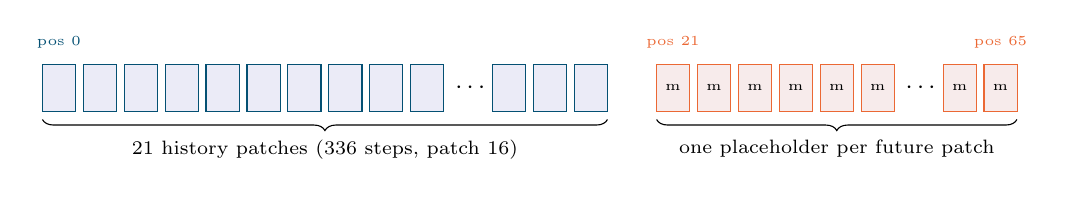
\begin{tikzpicture}[x=0.52cm,y=0.5cm,
  hist/.style={draw=blockhead,fill=blockbody,minimum width=0.42cm,minimum height=0.6cm,inner sep=0pt},
  fut/.style={draw=fixedc,fill=alertbody,minimum width=0.42cm,minimum height=0.6cm,inner sep=0pt}]
  \foreach \i in {0,...,9} \node[hist] (h\i) at (\i,0) {};
  \node at (10.1,0) {\small$\cdots$};
  \foreach \i in {11,...,13} \node[hist] (h\i) at (\i,0) {};
  \foreach \i in {15,...,20} \node[fut] (f\i) at (\i,0) {\tiny m};
  \node at (21.1,0) {\small$\cdots$};
  \foreach \i in {22,23} \node[fut] (f\i) at (\i,0) {\tiny m};
  \draw[decorate,decoration={brace,amplitude=4pt,mirror}] (-0.4,-0.8) -- (13.4,-0.8) node[midway,below=4pt]{\scriptsize 21 history patches (336 steps, patch 16)};
  \draw[decorate,decoration={brace,amplitude=4pt,mirror}] (14.6,-0.8) -- (23.4,-0.8) node[midway,below=4pt]{\scriptsize one placeholder per future patch};
  \node[above=2pt of f15,font=\tiny,fixedc] {pos 21};
  \node[above=2pt of f23,font=\tiny,fixedc] {pos 65};
  \node[above=2pt of h0,font=\tiny,blockhead] {pos 0};
\end{tikzpicture}
\vspace{0.25cm}
\begin{itemize}
\item 2-layer, 4-head Transformer encoder; $d=64$. Each history patch of 16 steps is one token.
\item All placeholders are the \textbf{same} learnable vector \texttt{m}: \textbf{only RoPE tells them apart}.
\item Mask: history sees history; a placeholder sees history and itself $\Rightarrow$ the forecast for step $h$ does not depend on $H$, so we can ask for \textbf{any} horizon after training.
\item Trained with $H=96$ (6 placeholders); queried with $H=720$ (45 placeholders).
\end{itemize}
\end{frame}

\begin{frame}{Our method: learnable frequency scales}
\begin{block}{Per-head learnable scale (the proposal's idea)}
\[
\hat\omega_{\ell,h,j}=\omega_j\cdot e^{a_{\ell,h}},\qquad a_{\ell,h}\ \text{learned, initialised at }0\ (=\text{standard RoPE})
\]
Only \textbf{4 extra parameters per layer} (one per head).
\end{block}
\textbf{Ablation variants} (to find out \emph{why} it works):
\begin{itemize}
\item \emph{Grouped}: separate scales for the fast and the slow frequency pairs.
\item \emph{Shared}: one scale for all heads of a layer.
\item \emph{Fixed}: scales set by hand and frozen (spread across heads, or aligned to the day).
\end{itemize}
\textbf{Second remedy --- multi-horizon training:} each batch uses $H\in\{96,192,336,720\}$, so one model also sees distant placeholders.
\end{frame}

\begin{frame}{Intuition: RoPE as a clock}
\begin{columns}[c]
\column{0.5\textwidth}
\centering
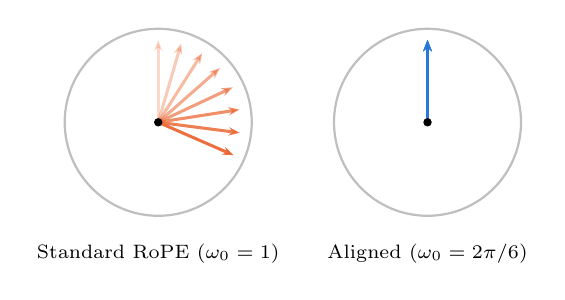
\begin{tikzpicture}[scale=0.95]
  \foreach \cx/\lab/\drift/\col in {0/{Standard RoPE ($\omega_0=1$)}/1/fixedc, 3.6/{Aligned ($\omega_0=2\pi/6$)}/0/learnc} {
    \draw[gray!50,thick] (\cx,0) circle (1.25);
    \node[font=\scriptsize,align=center] at (\cx,-1.75) {\lab};
    \foreach \k in {0,...,7} {
      \pgfmathsetmacro{\ang}{90 - \drift*\k*(2*pi-6)*180/pi}
      \pgfmathsetmacro{\op}{0.25+0.1*\k}
      \draw[\col,line width=1.1pt,opacity=\op,-{Stealth[length=4pt]}] (\cx,0) -- ++(\ang:1.1);
    }
    \fill (\cx,0) circle (1.6pt);
  }
\end{tikzpicture}
\\[2pt]{\scriptsize fastest hand at midnight on days 0--7 (darker = later)}
\column{0.48\textwidth}
\begin{itemize}
\item ETTm1: 15-min data, patch 16 $\Rightarrow$ \textbf{1 day = 6 tokens}.
\item Standard RoPE turns once per \textbf{6.28} tokens: it falls behind by 0.28 tokens a day.
\item Inside the training window the drift is small; 7 days ahead the hand points somewhere \textbf{never seen in training}.
\end{itemize}
\begin{block}{Alignment}
If $\hat\omega_0=2\pi/T$ ($T$ = tokens per day), position $t+T$ looks exactly like $t$: the far future looks like the past.
\end{block}
\end{columns}
\end{frame}

% ===================== Experiments =====================
\section{Experiments \& Mechanism}

\begin{frame}{Experimental setup}
\begin{columns}[T]
\column{0.5\textwidth}
\textbf{Data} (7 datasets, every variable its own series)
\begin{itemize}\small
\item Benchmarks: Electricity, ETTh1, ETTm1, Weather.
\item \textbf{Financial}: day-ahead electricity prices Nord Pool (EPF-NP) \& PJM (EPF-PJM); daily exchange rates.
\item Chronological splits; z-score on training rows only; RevIN for exchange rates.
\end{itemize}
\textbf{Metric:} MSE on the normalised scale.
\column{0.48\textwidth}
\textbf{Baselines \& why}
\begin{itemize}\small
\item \emph{Fixed RoPE}: same model without scales $\Rightarrow$ isolates the mechanism.
\item \emph{Linear} $\mathbb{R}^{336}\!\to\!\mathbb{R}^H$: as strong as Transformers here (DLinear).
\item \emph{Trained directly at 720}: the natural alternative to extrapolation.
\end{itemize}
\textbf{Protocol \& significance}
\begin{itemize}\small
\item Same backbone, paired seeds, base and checkpoint chosen on validation only.
\item 3--5 seeds + \textbf{Diebold--Mariano} test (Newey--West, overlapping windows).
\end{itemize}
\end{columns}
\end{frame}

\begin{frame}{Result 1: at the training horizon}
\centering\small
\begin{tabular}{lccc}\toprule
Test MSE, $H=96$ & Linear & Transformer, fixed RoPE & Transformer, learnable scale\\\midrule
Electricity & 0.140 & 0.139 & 0.139\\
ETTh1 & \textbf{0.377} & 0.417 & 0.414\\
ETTm1 & \textbf{0.304} & 0.311 & 0.317\\
Weather & 0.174 & \textbf{0.153} & \textbf{0.153}\\
EPF-NP & 0.472 & 0.482 & \textbf{0.452}\\
EPF-PJM & \textbf{0.163} & 0.174 & 0.167\\
Exchange & \textbf{0.089} & 0.103 & 0.099\\\bottomrule
\end{tabular}
\vspace{0.3cm}
\begin{itemize}
\item The Transformer is close to published results (PatchTST/42: Electricity 0.130, Weather 0.152).
\item Linear models remain strong (as reported by DLinear).
\item Fixed vs.\ learnable differ by about one seed std or less here --- the main effect lies \textbf{beyond} the horizon.
\end{itemize}
\end{frame}

\begin{frame}{Result 2: fixed RoPE degrades beyond it}
\begin{columns}[c]
\column{0.7\textwidth}\centering
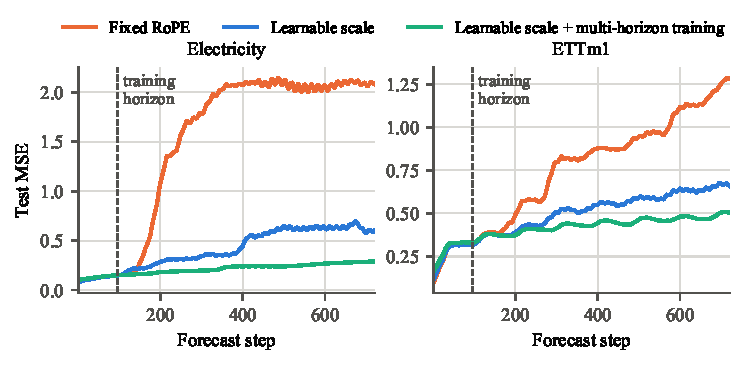
\includegraphics[width=\textwidth]{figs/fig1_perstep.pdf}\\
{\scriptsize Test MSE per forecast step; trained at $H=96$ (dashed line).}
\column{0.28\textwidth}\centering
{\huge\bfseries\color{fixedc}6.4$\times$}\\{\scriptsize error of fixed RoPE at 720 steps vs.\ a model trained at 720 (Electricity)}\\[0.35cm]
{\huge\bfseries\color{learnc}38--66\%}\\{\scriptsize lower error with learnable scales (Electricity, ETTh1, ETTm1)}\\[0.35cm]
{\huge\bfseries\color{navy}6\,/\,6}\\{\scriptsize runs improve, each significant (Diebold--Mariano), on all three}
\end{columns}
\end{frame}

\begin{frame}{Result 2: all datasets at 720 steps}
\centering\scriptsize
\setlength{\tabcolsep}{4pt}
\begin{tabular}{lcccccc}\toprule
& \multicolumn{2}{c}{Trained at 96, asked for 720} & DM & Multi-horizon & \multicolumn{2}{c}{Trained at 720}\\
\cmidrule(lr){2-3}\cmidrule(lr){6-7}
Test MSE, steps 1--720 & fixed & learnable & $+\,/\,-$ & learnable & Transformer & Linear\\\midrule
\inputtab tables/t2_extrap.tex
\bottomrule\end{tabular}
\vspace{0.3cm}
\begin{itemize}\small
\item Strong, significant gains on seasonal data: Electricity, ETTh1, ETTm1 and \textbf{both electricity markets}.
\item No consistent gain on Weather and Exchange rates (DM results of mixed sign) --- explained on the next slides.
\item DM column: of 6 runs (3 seeds $\times$ 2 bases), how many are significantly better\,/\,worse ($p<0.05$).
\end{itemize}
\end{frame}

\begin{frame}{Why: alignment to the daily cycle}
\begin{columns}[c]
\column{0.52\textwidth}
\centering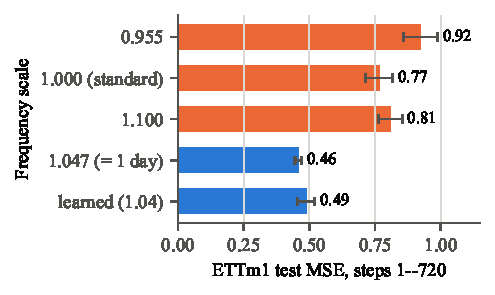
\includegraphics[width=0.95\textwidth]{figs/fig2_alignment.pdf}
\column{0.46\textwidth}
\begin{itemize}
\item ETTm1: 1 day = 6 tokens $\Rightarrow$ aligned scale $2\pi/6=\mathbf{1.047}$.
\item Learned scales average \textbf{1.04} --- in both layers.
\item \textbf{Fixed at 1.047, no learning}: matches the learned model.
\item 5\% too slow (0.955) or fast (1.10): degrades like standard RoPE.
\item DM test 1.047 vs 0.955: $p<10^{-15}$ in 6/6 runs.
\end{itemize}
\end{columns}
\begin{alertblock}{Explanation supported by the evidence}
Learning helps by moving \textbf{RoPE's fastest rotation close to the daily cycle}.
\end{alertblock}
\end{frame}

\begin{frame}{Attention: what the placeholders look at}
\centering
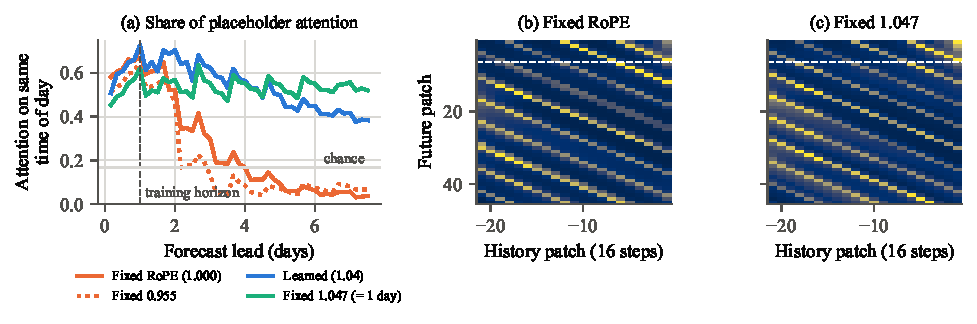
\includegraphics[width=0.8\textwidth]{figs/fig4_attention.pdf}\\[-3pt]
{\tiny ETTm1, trained at $H=96$, queried at 720; last layer, mean of 3 seeds; dashed line = training horizon.}
\begin{itemize}\footnotesize
\item Future patches attend to history at the \textbf{same time of day} (stripes every 6 patches): a ``same time yesterday'' lookup.
\item \textbf{Fixed RoPE loses it} after $\sim$2 days ($0.64\to0.05$, below chance); \textbf{aligned 1.047 keeps it} ($\approx0.53$); learned 1.04 decays slowly.
\end{itemize}
\end{frame}



\begin{frame}{Gain grows with the daily cycle}
\centering
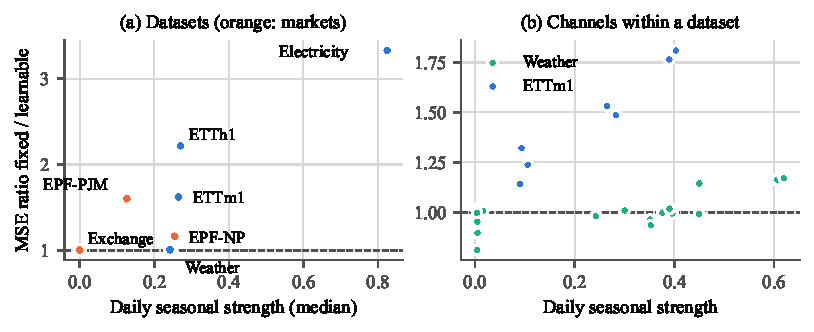
\includegraphics[width=0.86\textwidth]{figs/fig3_periodicity.pdf}
\begin{itemize}\small
\item \textbf{Datasets}: strongest cycle (Electricity) gains most; no cycle (Exchange): no consistent effect.
\item \textbf{Channels}: in Weather only the 3 solar-radiation channels gain --- so Weather as a whole shows none.
\end{itemize}
\end{frame}

\begin{frame}{Remedy 2: multi-horizon training}
\begin{columns}[c]
\column{0.5\textwidth}
\centering\small
\begin{tabular}{lccc}\toprule
MSE, 720 steps & Learnable & Multi-H & Trained\\
& @96 & (1 model) & @720\\\midrule
Electricity & 0.464 & \textbf{0.216} & 0.210\\
ETTm1 & 0.474 & \textbf{0.421} & 0.435\\
Weather & 0.396 & \textbf{0.326} & 0.336\\
EPF-PJM & 0.273 & \textbf{0.216} & 0.213\\
ETTh1 & \textbf{0.473} & 0.541 & 0.632\\
EPF-NP & \textbf{0.896} & 1.123 & 1.196\\\bottomrule
\end{tabular}
\column{0.48\textwidth}
\begin{itemize}\small
\item One model trained on mixed horizons is within 3\% of, or better than, the model trained at 720 --- on \textbf{all 7 datasets}.
\item Small cost at $H=96$ (Electricity 0.135 vs 0.128).
\item With it, fixed and learnable RoPE perform alike (distant positions are seen in training).
\item When long-horizon training \textbf{overfits} (small ETTh1, noisy EPF-NP), learnable scales + extrapolation do better.
\end{itemize}
\end{columns}
\end{frame}

% ===================== Finance =====================
\section{Application to Finance}

\begin{frame}{Application to finance}
\begin{columns}[T]
\column{0.5\textwidth}
\begin{block}{Electricity markets (daily cycle)}
\small Learnable scales cut 720-step error significantly:\\
EPF-PJM $0.44\to\mathbf{0.27}$ (6/6 runs),\\
EPF-NP $1.07\to\mathbf{0.90}$ (5/6 runs).
\end{block}
\column{0.46\textwidth}
\begin{block}{Exchange rates (random walk)}
\small No cycle to align $\Rightarrow$ no consistent effect (3 better, 3 worse); linear model best; RevIN essential.
\end{block}
\end{columns}
\vspace{0.2cm}
\begin{alertblock}{Practical guidance from our results}
\begin{enumerate}\small
\item For \textbf{seasonal} financial series --- intraday volume \& volatility (daily U-shape), power \& gas prices --- use learnable or calendar-aligned RoPE before forecasting beyond the training horizon.
\item To cover several risk horizons (1- \& 10-day VaR, HAR-style volatility) with \textbf{one model}, train on mixed horizons.
\item For near-random-walk prices, we saw no benefit from position encodings.
\end{enumerate}
\end{alertblock}
\end{frame}

% ===================== Conclusion =====================
\section{Limitations \& Takeaways}

\begin{frame}{Limitations \& future work}
\textbf{What did not work / limitations}
\begin{itemize}
\item No evidence that heads specialise to distinct time scales (the proposal's hypothesis).
\item Mechanism analyses cover ETTh1, ETTm1 and Weather only.
\item Grouping frequencies (the starting repository's hypothesis) gave no extra gain.
\item Small model (2 layers, $d=64$), 3--5 seeds (partly offset by DM tests).
\item With point tokens instead of patches the effect is much noisier; linear models stay strong at the training horizon.
\end{itemize}
\textbf{Future work}
\begin{itemize}
\item Initialise frequencies from the data's dominant period (FFT) instead of learning them.
\item Align several frequencies to several cycles (day \emph{and} week).
\item Test on larger Transformers and time-series foundation models that use RoPE.
\end{itemize}
\end{frame}

\begin{frame}{Takeaways}
\vspace{-0.15cm}
\begin{block}{1. The problem}
In our experiments, RoPE forecasters trained at one horizon \textbf{degrade sharply} beyond it: up to $6.4\times$ the error of a directly trained model.
\end{block}
\begin{block}{2. The likely cause}
RoPE's rotation is \textbf{out of step with the daily cycle}; far-ahead positions look unlike those seen in training.
\end{block}
\begin{block}{3. The remedies}
4 learnable scales per layer \textbf{align} it (38--66\% less error, consistent across runs); one \textbf{mixed-horizon} model comes within 3\% of per-horizon models.
\end{block}
\begin{alertblock}{For finance}
Helped on seasonal markets (electricity prices); no consistent effect on random-walk prices (exchange rates).
\end{alertblock}
\end{frame}

\begin{frame}[plain]
  \centering
  \Large \textbf{Thank you!}\\[0.5cm]
  \normalsize Questions?
\end{frame}

% ===================== Backup =====================
\appendix

\begin{frame}{Backup: What Does \emph{Not} Matter}
\begin{columns}[c]
\column{0.5\textwidth}
\centering\footnotesize
\begin{tabular}{@{}lc@{}}\toprule
Frequency scales & Test MSE\\\midrule
\inputtab tables/t3_mechanism.tex
\bottomrule\end{tabular}
\column{0.48\textwidth}
\begin{itemize}\small
\item \textbf{Head diversity}: for extrapolation, one shared scale performs as well as one per head; hand-set spreads help little or hurt.\\$\Rightarrow$ no evidence the gain needs head specialisation.
\item \textbf{Grouping}: the fast group learns the same value as the per-head scale; the slow group drifts with no measurable effect.\\$\Rightarrow$ the effect sits in the \textbf{fast} frequencies.
\item \textbf{Gradient clipping}: inactive after warm-up, so not the cause.
\end{itemize}
\end{columns}
\end{frame}

\begin{frame}{Backup: Transformer Basics}
\small
\begin{columns}[T]   % Top-aligned columns
  % -------- Left column --------
  \column{0.54\textwidth}
  \textbf{Architecture.} Standard encoder–decoder with positional encodings (Vaswani et al., 2017).

  \medskip
  \textbf{Tokenization.} History as tokens $\{x_1,\ldots,x_L\}$ (points or patches).

\textbf{Projections.}\quad
$Q=XW_Q,\ \ K=XW_K,\ \ V=XW_V\ \ (\in\mathbb{R}^{L\times d})$

\vspace{-0.2cm}  % 往上挪一丢丢

\begin{block}{\centering \textbf{Scaled dot-product attention (key equation)}}
\[
\mathrm{Attn}(Q,K,V)=
\mathrm{Softmax}\!\left(\frac{QK^{\top}}{\sqrt{d}}\right)V
\]
\end{block}

  \vspace{2pt}
  Multi-head attention allows different heads to capture diverse temporal patterns.  
  Stacking layers builds contextual representations for sequence prediction.

  % -------- Right column --------
  \column{0.44\textwidth}
  \centering
  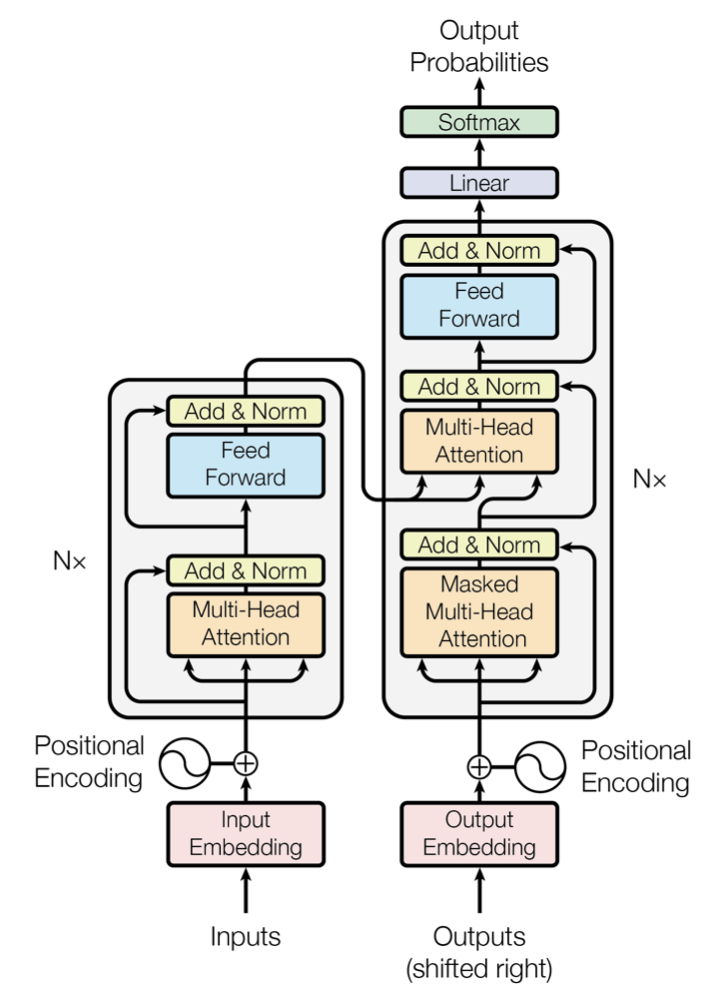
\includegraphics[width=0.95\linewidth,height=0.75\textheight,keepaspectratio]{figs/transformer_architecture.png}
\end{columns}
\end{frame}

\begin{frame}{Backup: Positional Encoding}
\small
\begin{block}{Why do we need position encodings?}
Self-attention treats the input as an unordered set of tokens —  
without additional signals, it cannot tell which time step comes first.
\end{block}

\begin{itemize}
  \item To restore temporal order, each token $x_\ell$ is added with a \textbf{positional encoding}:
  \[
  \tilde{x}_\ell = x_\ell + PE(\ell).
  \]
  \item The encoding $PE(\ell)$ can be:
  \begin{itemize}
    \item \textbf{Sinusoidal:} fixed periodic functions $\sin(\omega \ell), \cos(\omega \ell)$ (Vaswani et al., 2017).
    \item \textbf{Learnable:} parameters trained with the model (BERT-style).
  \end{itemize}
  \item This addition injects absolute position information into the input before attention.
\end{itemize}

\begin{alertblock}{RoPE's idea}
RoPE \textbf{replaces this absolute positional addition step}  
with a \textbf{rotation-based operation} inside the attention itself —  
making the attention score aware of relative offsets instead of absolute indices.
\end{alertblock}
\end{frame}

\begin{frame}{Backup: Why Relative Positions}
\small
\begin{itemize}
  \item In NLP, \textbf{absolute positions} work because word order carries meaning.
  \item In time-series forecasting, especially in \textbf{financial data}, we care more about \textbf{relative offsets}:
    \begin{itemize}
      \item Forecasting at $t{+}1$ should be invariant to where the window starts — the market pattern ``5 days before a crash'' should look the same in 2018 or 2024.
      \item Temporal similarity depends on \textbf{distance $\Delta$}, not on the absolute calendar index $\ell$.
      \item Financial series are often non-stationary — absolute time (e.g., day 2000 vs. day 4000) has little predictive meaning.
    \end{itemize}

\end{itemize}

\begin{alertblock}{Motivation for RoPE}
\vspace{-1mm}
\centering
\[
\underbrace{
\begin{aligned}
q_m &= f_q(x_m,\, m),\\
k_n &= f_k(x_n,\, n)
\end{aligned}
}_{\text{absolute position encoding}}
\quad
\Longrightarrow
\quad
\underbrace{
\langle f_q(x_m,m), f_k(x_n,n) \rangle
= g(x_m, x_n,\, m-n)
}_{\text{relative position encoding target}}
\]
\vspace{-1mm}
\end{alertblock}
\end{frame}

\begin{frame}{Backup: From Rotation to Relative Encoding}
\footnotesize
\textbf{Setup.}
Let $d_h$ be even, $m=d_h/2$.
Split $q,k\in\mathbb{R}^{d_h}$ into 2D blocks:
\[
q=[q^{(0)};\ldots;q^{(m-1)}],\quad
k=[k^{(0)};\ldots;k^{(m-1)}],\quad
q^{(i)},k^{(i)}\in\mathbb{R}^2.
\]

\textbf{RoPE rotation.}
\[
R(\omega_i \ell)=
\begin{bmatrix}
\cos(\omega_i \ell)&-\sin(\omega_i \ell)\\
\sin(\omega_i \ell)&\cos(\omega_i \ell)
\end{bmatrix},\quad
q'^{(i)}=R(\omega_i\ell_q)q^{(i)},\;
k'^{(i)}=R(\omega_i\ell_k)k^{(i)}.
\]

\textbf{Dot-product score:}
\[
S=\frac{(q')^\top k'}{\sqrt{d_h}}
=\frac{1}{\sqrt{d_h}}\sum_{i=0}^{m-1}{q'^{(i)}}^\top k'^{(i)}.
\]

\begin{block}{Goal}
Show $S$ can be rewritten as a function of the \textbf{relative offset} 
$\Delta=\ell_k-\ell_q$.
\end{block}
\end{frame}

\begin{frame}{Backup: Trigonometric Foundation of RoPE}
\footnotesize

\textbf{Rotation matrix:} 
\(
R(\theta)=
\begin{bmatrix}
\cos\theta & -\sin\theta\\
\sin\theta & \cos\theta
\end{bmatrix}.
\)

\vspace{1mm}
\textbf{Compute:}
\[
R(\alpha)^\top R(\beta)
=
\begin{bmatrix}
\cos\alpha & \sin\alpha\\[-2pt]
-\sin\alpha & \cos\alpha
\end{bmatrix}
\!\!
\begin{bmatrix}
\cos\beta & -\sin\beta\\[-2pt]
\sin\beta & \cos\beta
\end{bmatrix}.
\]

\vspace{1mm}
\textbf{Multiplication result:}
\[
\!\!=
\begin{bmatrix}
\cos\alpha\cos\beta+\sin\alpha\sin\beta &
-\cos\alpha\sin\beta+\sin\alpha\cos\beta\\[-1pt]
-\sin\alpha\cos\beta+\cos\alpha\sin\beta &
\sin\alpha\sin\beta+\cos\alpha\cos\beta
\end{bmatrix}.
\]

\vspace{1mm}
\textbf{Apply trig identities:}
\[
\begin{cases}
\cos(\beta-\alpha)=\cos\beta\cos\alpha+\sin\beta\sin\alpha,\\[-2pt]
\sin(\beta-\alpha)=\sin\beta\cos\alpha-\cos\beta\sin\alpha,
\end{cases}
\]

\vspace{1mm}
\textbf{Hence:}
\[
R(\alpha)^\top R(\beta)
=
\begin{bmatrix}
\cos(\beta-\alpha) & -\sin(\beta-\alpha)\\[-1pt]
\sin(\beta-\alpha) & \cos(\beta-\alpha)
\end{bmatrix}
=R(\beta-\alpha).
\]

\vspace{1mm}
Composing two rotations equals a single rotation 
by the \textbf{angle difference} $(\beta-\alpha)$ — 
the key property enabling RoPE’s relative encoding.
\end{frame}

\begin{frame}{Backup: Relative Dependence Emerges}
\footnotesize
\textbf{Key trigonometric identity.}
\[
R(\alpha)^\top R(\beta)=R(\beta-\alpha)
\quad\Longleftrightarrow\quad
\begin{cases}
\cos(\beta-\alpha)=\cos\beta\cos\alpha+\sin\beta\sin\alpha,\\[3pt]
\sin(\beta-\alpha)=\sin\beta\cos\alpha-\cos\beta\sin\alpha.
\end{cases}
\]

\textbf{Apply to RoPE rotations.}
\[
{q'^{(i)}}^\top k'^{(i)}
=(R(\omega_i \ell_q)q^{(i)})^\top (R(\omega_i \ell_k)k^{(i)})
={q^{(i)}}^\top R(\omega_i(\ell_k-\ell_q))k^{(i)}.
\]

\textbf{Therefore}
\[
\boxed{%
S(\Delta)=\tfrac{1}{\sqrt{d_h}}
\sum_{i=0}^{m-1}{q^{(i)}}^\top R(\omega_i\Delta)k^{(i)}},
\qquad
\Delta=\ell_k-\ell_q.
\]

\textit{Here the trigonometric identity merges the query and key rotations 
into a single relative rotation $R(\omega_i\Delta)$, 
so each 2D block interacts only through the relative offset $\Delta$.}
\end{frame}

\begin{frame}{Backup: replication \& hyper-parameters}
\small
\begin{itemize}
\item Code: \texttt{github.com/ycsama0703/ft5011-ropeformer} + \texttt{experiments/} (commands in \texttt{experiments/README.md}).
\item Data: Time-Series-Library (HuggingFace, CC BY 4.0); EPF (Zenodo 4624805); exchange rates (Time-Series-Library).
\item $L=336$, patch 16, $d=64$, 4 heads, 2 layers, FFN 128, dropout 0.1, batch 256.
\item AdamW, lr $10^{-3}$ (no weight decay on scales), 300 warm-up steps + cosine, clip 1.0, bf16.
\item Budgets: 2000 steps (ETTh1, EPF, exchange), 4000 (ETTm1), 6000 (Weather), 8000 (Electricity).
\item RoPE base $\in\{10^3,10^4\}$ and best checkpoint chosen on validation; test used once.
\item One run: 20 s -- 3 min on one H100 (memory capped at 8\%).
\end{itemize}
\end{frame}

\end{document}
